%% Write your code here.
\documentclass{beamer}
\usepackage[spanish]{babel}
\usepackage[utf8]{inputenc}
\usepackage[T1]{fontenc}
\usepackage{amsmath,amssymb,amsfonts}
\usepackage{xcolor}
\usepackage{biblatex}
\usepackage{ragged2e}
\usepackage{hyperref}
\usepackage{etoolbox}
\usepackage{lipsum}
\usepackage[center]{caption}

\newcommand\blfootnote[1]{%
  \begingroup
  \renewcommand\thefootnote{}\footnote{#1}%
  \addtocounter{footnote}{-1}%
  \endgroup
}

\addbibresource{biblio.bib}

\usetheme{Madrid}
\title{Teorías de estructura espiral}
\author[Alfonso, Jacobo y Luis]{Alfonso de Lucas Iniesta, Jacobo Ruiz Morales y Luis Lucas García}
\institute[UA]{Universidad de Alicante}
\date{17 de mayo de 2024}

\apptocmd{\frame}{}{\justifying}{}

\begin{document}
\begin{frame}
\titlepage
\end{frame}

\begin{frame}
\frametitle{Tabla de contenidos}
\tableofcontents
\end{frame}

\begin{frame}{Motivación}
\section{Motivación}
Aproximadamente el 60\% de las galaxias son espirales. Dentro de este grupo el 10\% son de gran estructura, el 60\% de multiples brazos y el 30\% las floculentas. \cite{spiral}

\begin{alertblock}{Pregunta}
¿Cómo podemos explicar la formación de estas estructuras en las galaxias?
\end{alertblock}

\begin{figure}[h!]
\label{fig1}
     \begin{center}
     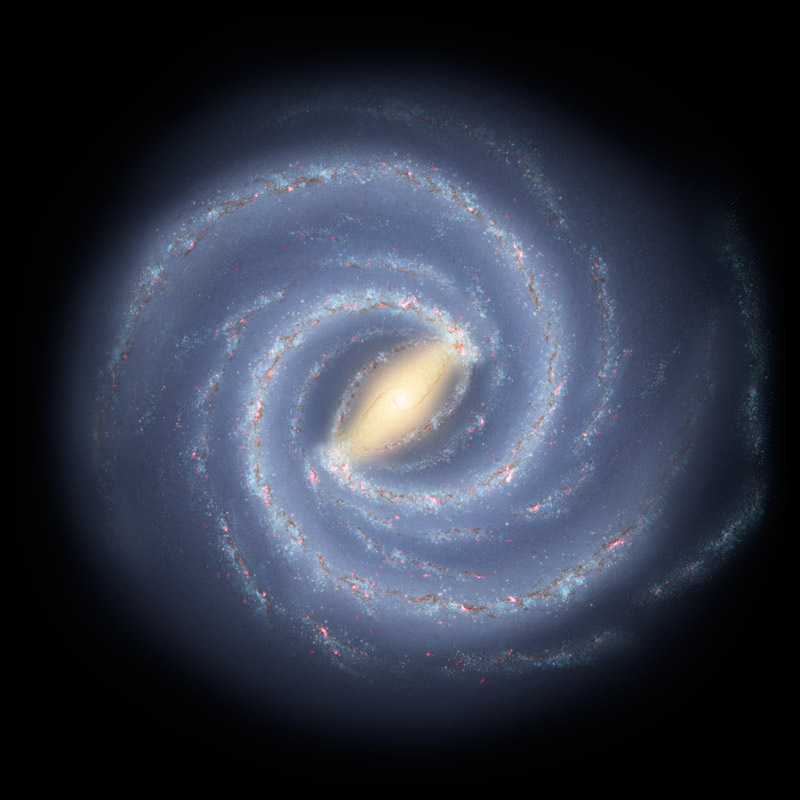
\includegraphics[scale=0.09]{multipleArms.jpg}
     \hspace{0.5cm}
     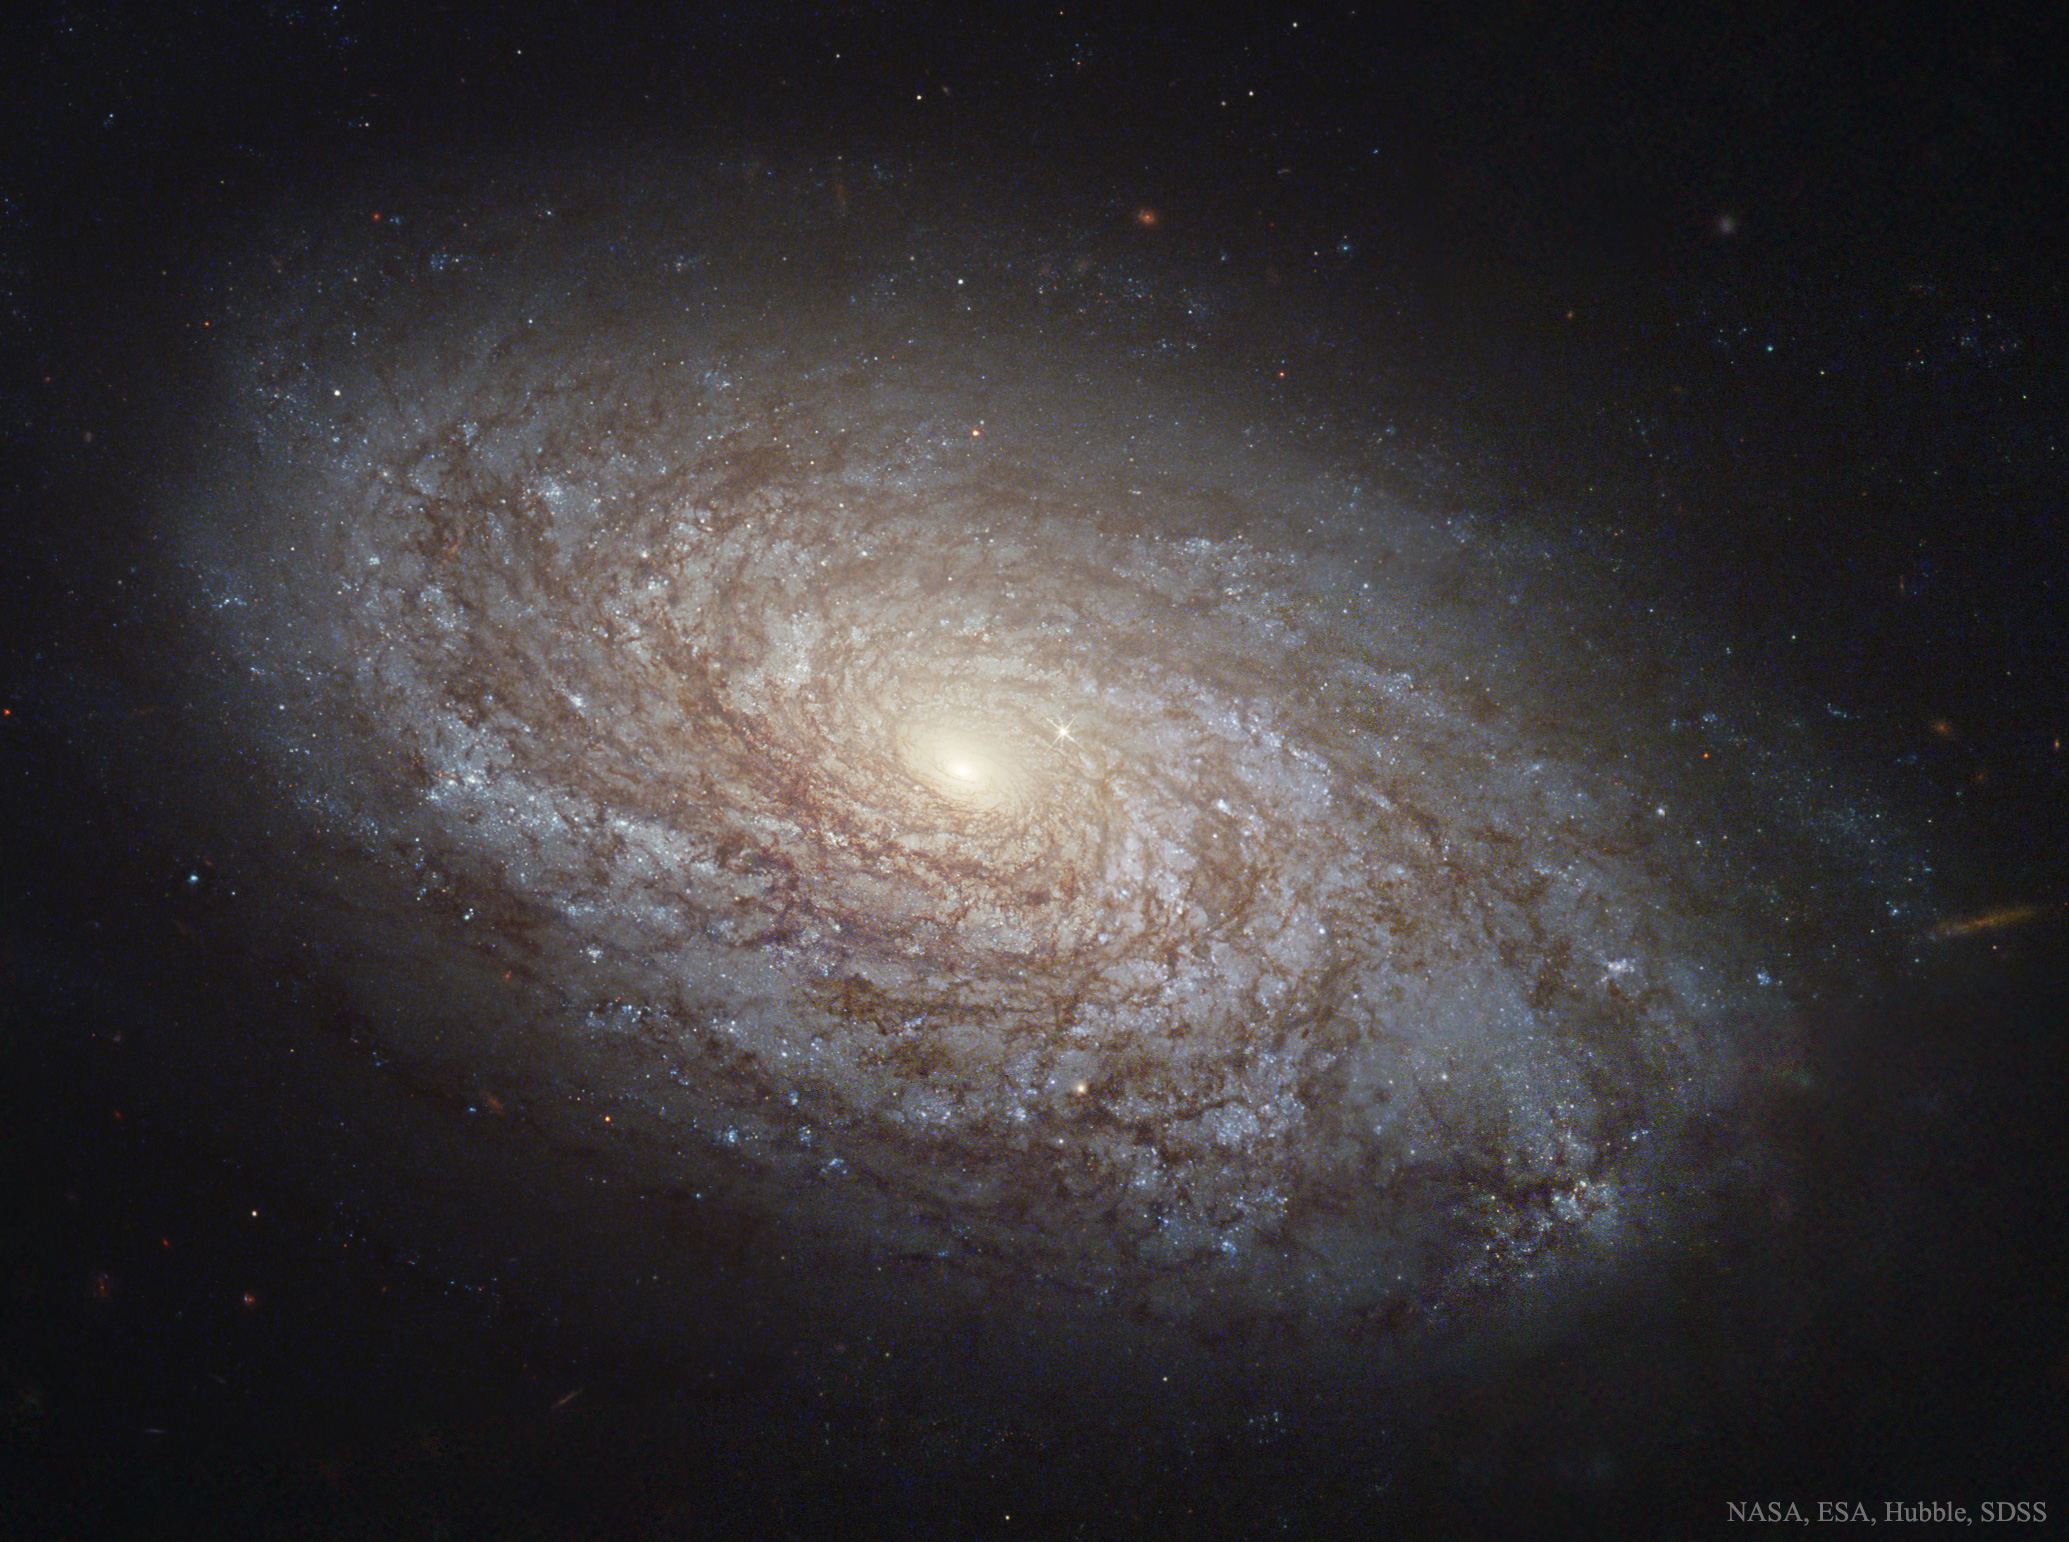
\includegraphics[scale=0.05]{floculenta.jpg}
     \hspace{0.5cm}
     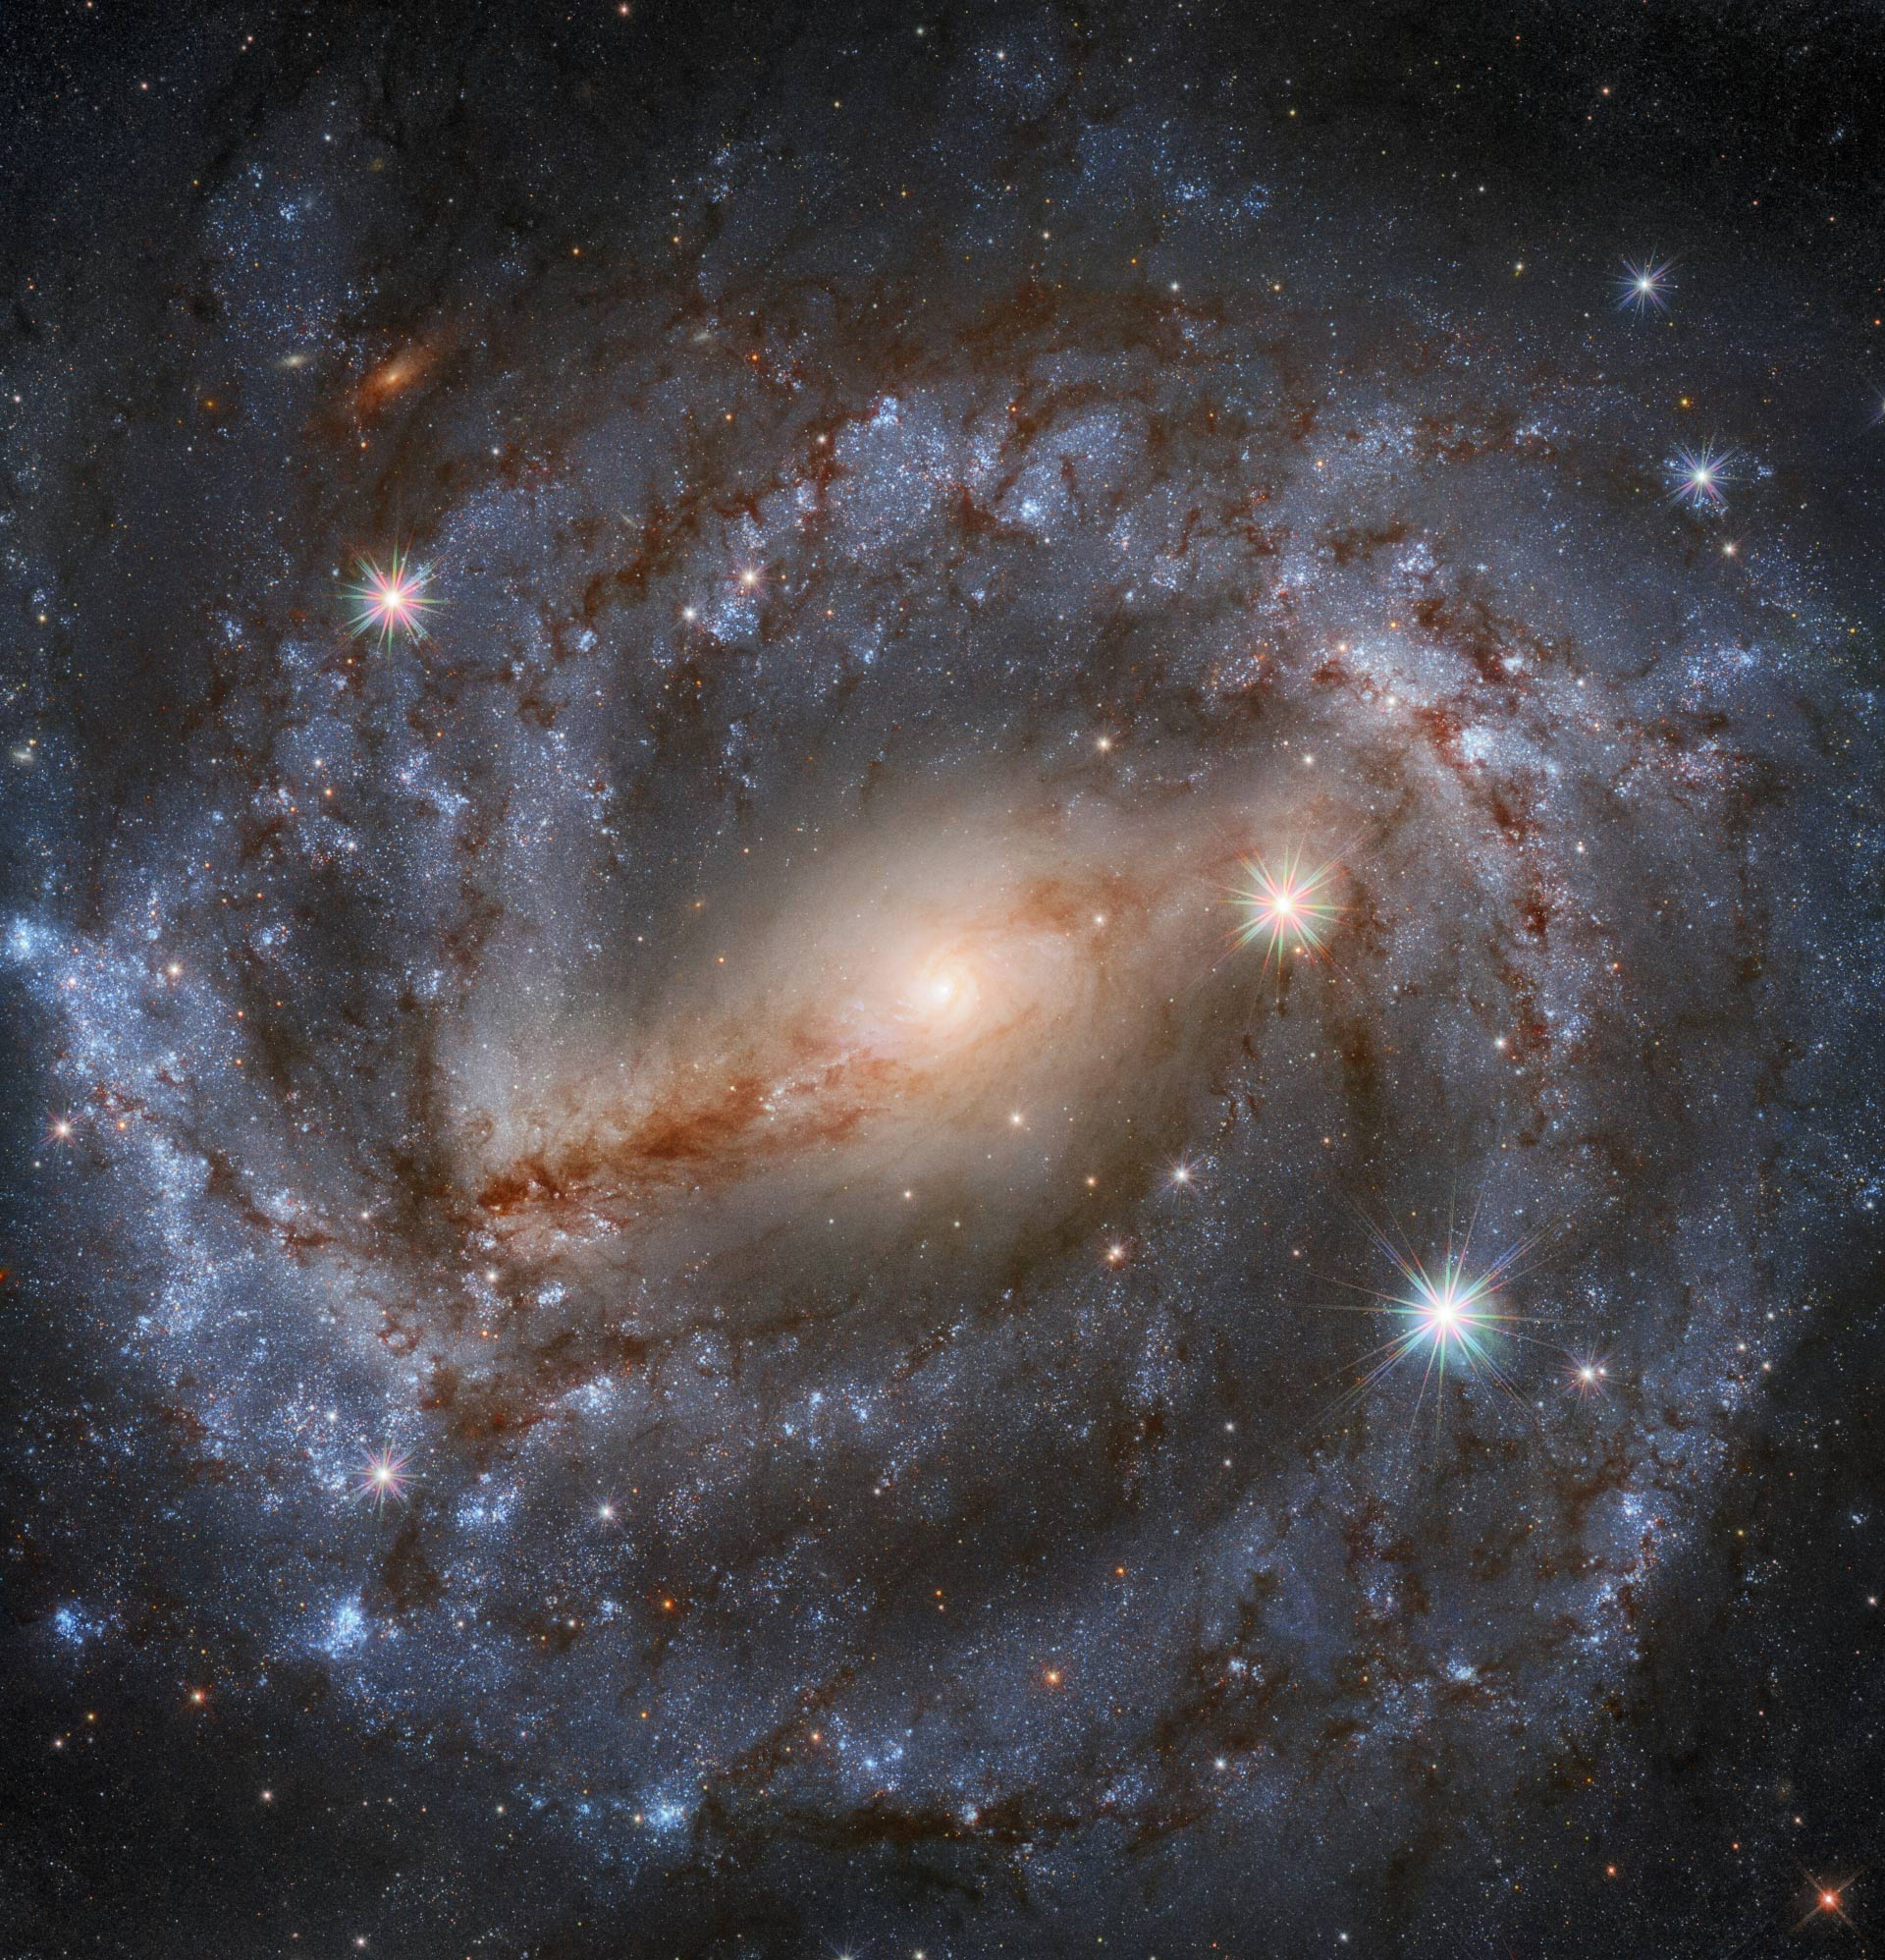
\includegraphics[scale=0.04]{granDiseno.jpg}
     \caption{Una galaxia de brazos múltiples, floculenta y de gran diseño respectivamente.}
     \end{center}
\end{figure}
\end{frame}

\begin{frame}{Dos modelos simples}

 \begin{block}{Modelo de sólido rígido}
 Suponiendo una velocidad angular constante como en cualquier sólido rígido podemos ver la velocidad lineal:
 
 $$
 v = \omega r
 $$
 \end{block}
 \begin{block}{Rotación diferencial}
 Suponiendo que la velocidad lineal es constante podemos tener una velocidad angular:
 
 $$
 \omega = \frac{v}{r}
 $$
 \end{block}
 
 El primer modelo no forma brazos y parece ser un molinillo rígido. Esto obviamente no es una estructura espiral válida.

\end{frame}

\begin{frame}{Simulaciones}
\url{https://github.com/luisgotsky} \cite{github}
\end{frame}

\begin{frame}
Aun así, vemos galaxias espirales de múltiples rango de edades:

\begin{figure}[h!]
\label{fig2}
    \begin{center}
    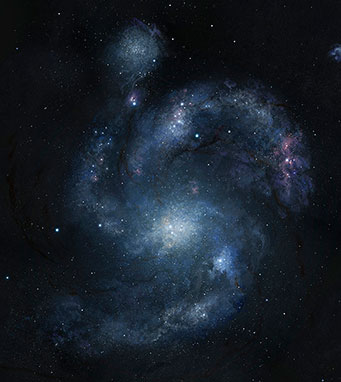
\includegraphics[scale=0.23]{sn-spiral.jpg}
    \hspace{0.5cm}
    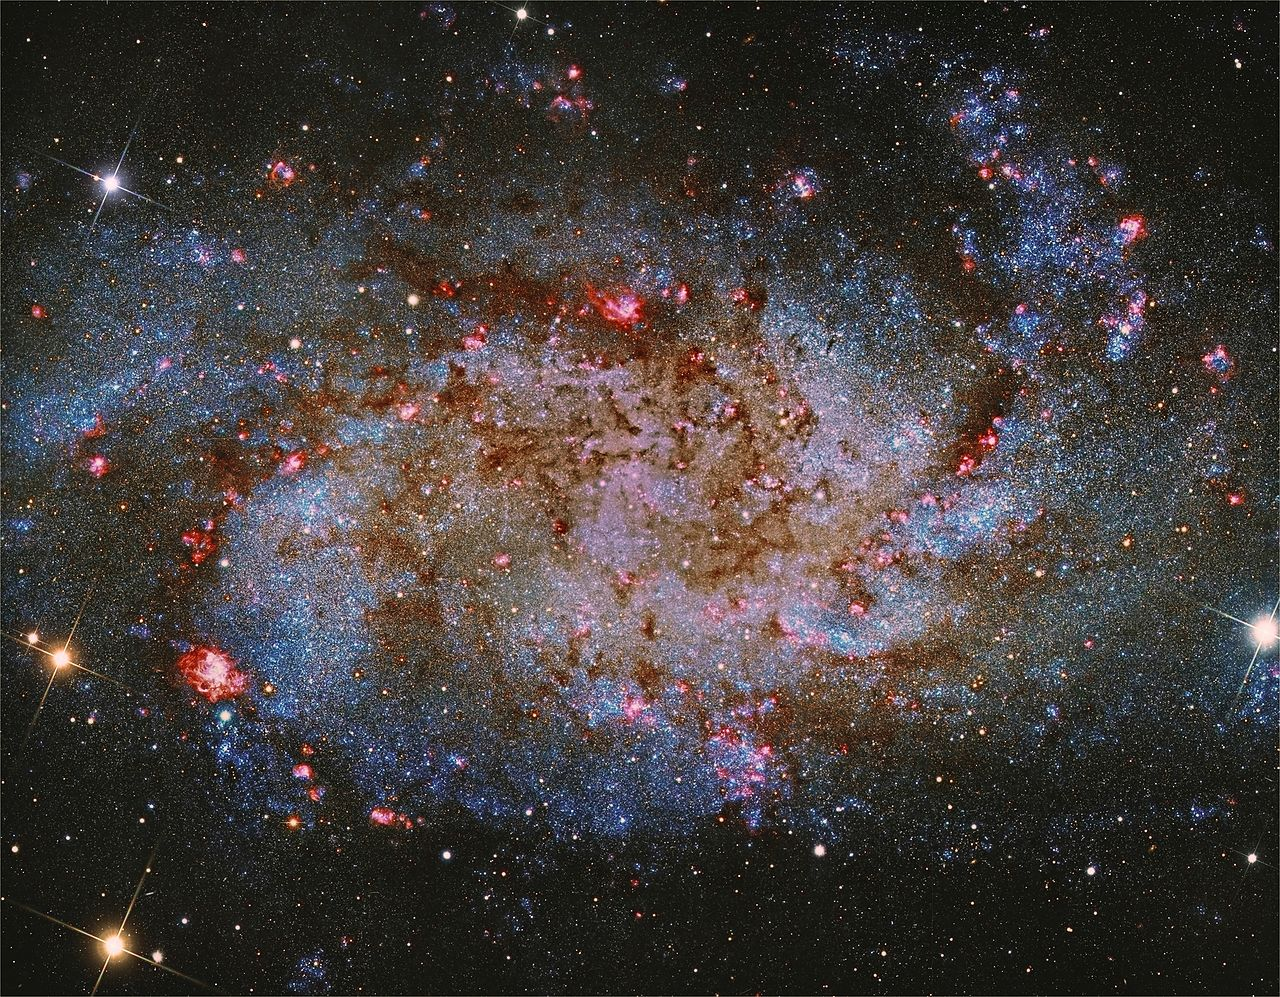
\includegraphics[scale=0.088]{Messier_33}
    \caption{Estructura espiral de BX442 y Messier 33.}
    \end{center}
\end{figure}

\begin{alertblock}{}
Entonces, ¿por qué seguimos viendo los brazos?
\end{alertblock}

\end{frame}

\begin{frame}{Un modelo más válido}
\section{Diferentes acercamientos}
\begin{block}{Ondas de densidad}
Actualmente, el modelo más aceptado es el de densidades de ondas, propuesto originalmente en la década de los 60  por los astrónomos Chia Chiao Lin y Frank Shu. Aunque se ha ido modificando con los años. \cite{LinShu}.
\end{block}
Estas ondas son estructuras cuasiestáticas densas y que avanzan lentamente.
\begin{itemize}
    \item Las estrellas y nubes del disco atravesarán los brazos.%Con distintas velocidades
    \item Las estrellas masivas nacerán y morirán rápidamente.%(brillo de la estructura)
    \item En cambio, las estrellas más comedidas escaparán de la estructura.
\end{itemize}
\end{frame}

\begin{frame}{Simulación con ondas de densidad}
%Aquí metería una simulación enseñando la dinámica de una galaxia basada en la teoría de las ondas de densidad, viendo cómo las estrella entran y salen de las zonas densas
\url{https://beltoforion.de/en/spiral_galaxy_renderer/}
\end{frame}
\begin{frame}{¿Por qué se forman estas ondas?}

Tenemos varias hipótesis sobre la formación de esta onda de densidad:

\begin{block}{Asimetría inicial}
Una asimetría inicial, que genere un desbalance de masa, podría dar inicio al movimiento de la onda de densidad.
\end{block}
\begin{block}{Posesión de una barra central}
La barra central de algunas galaxias puede provocar una perturbación gravitacional lo suficientemente grande como para generar densidades del tipo espiral.
\end{block}
\begin{block}{Interacción con otra galaxia}
Si la galaxia interactúa con sus galaxias vecinas o alguna pasante, una perturbación puede cambiar la estructura de la galaxia, dando inicio a una onda de densidad. %Esto se aprecia en \href{https://www.youtube.com/watch?v=lMReQ6hVw5s}{esta simulación}.
\end{block}

\end{frame}
\begin{frame}{¿Qué pasa con las Galaxias Floculentas?}

\begin{alertblock}{Galaxias floculentas}
Las simulaciones tienden a formar galaxias de Gran Diseño, aunque en el universo observamos patrones más complejos como las floculentas.
\end{alertblock}

\begin{figure}[h!]
\begin{center}
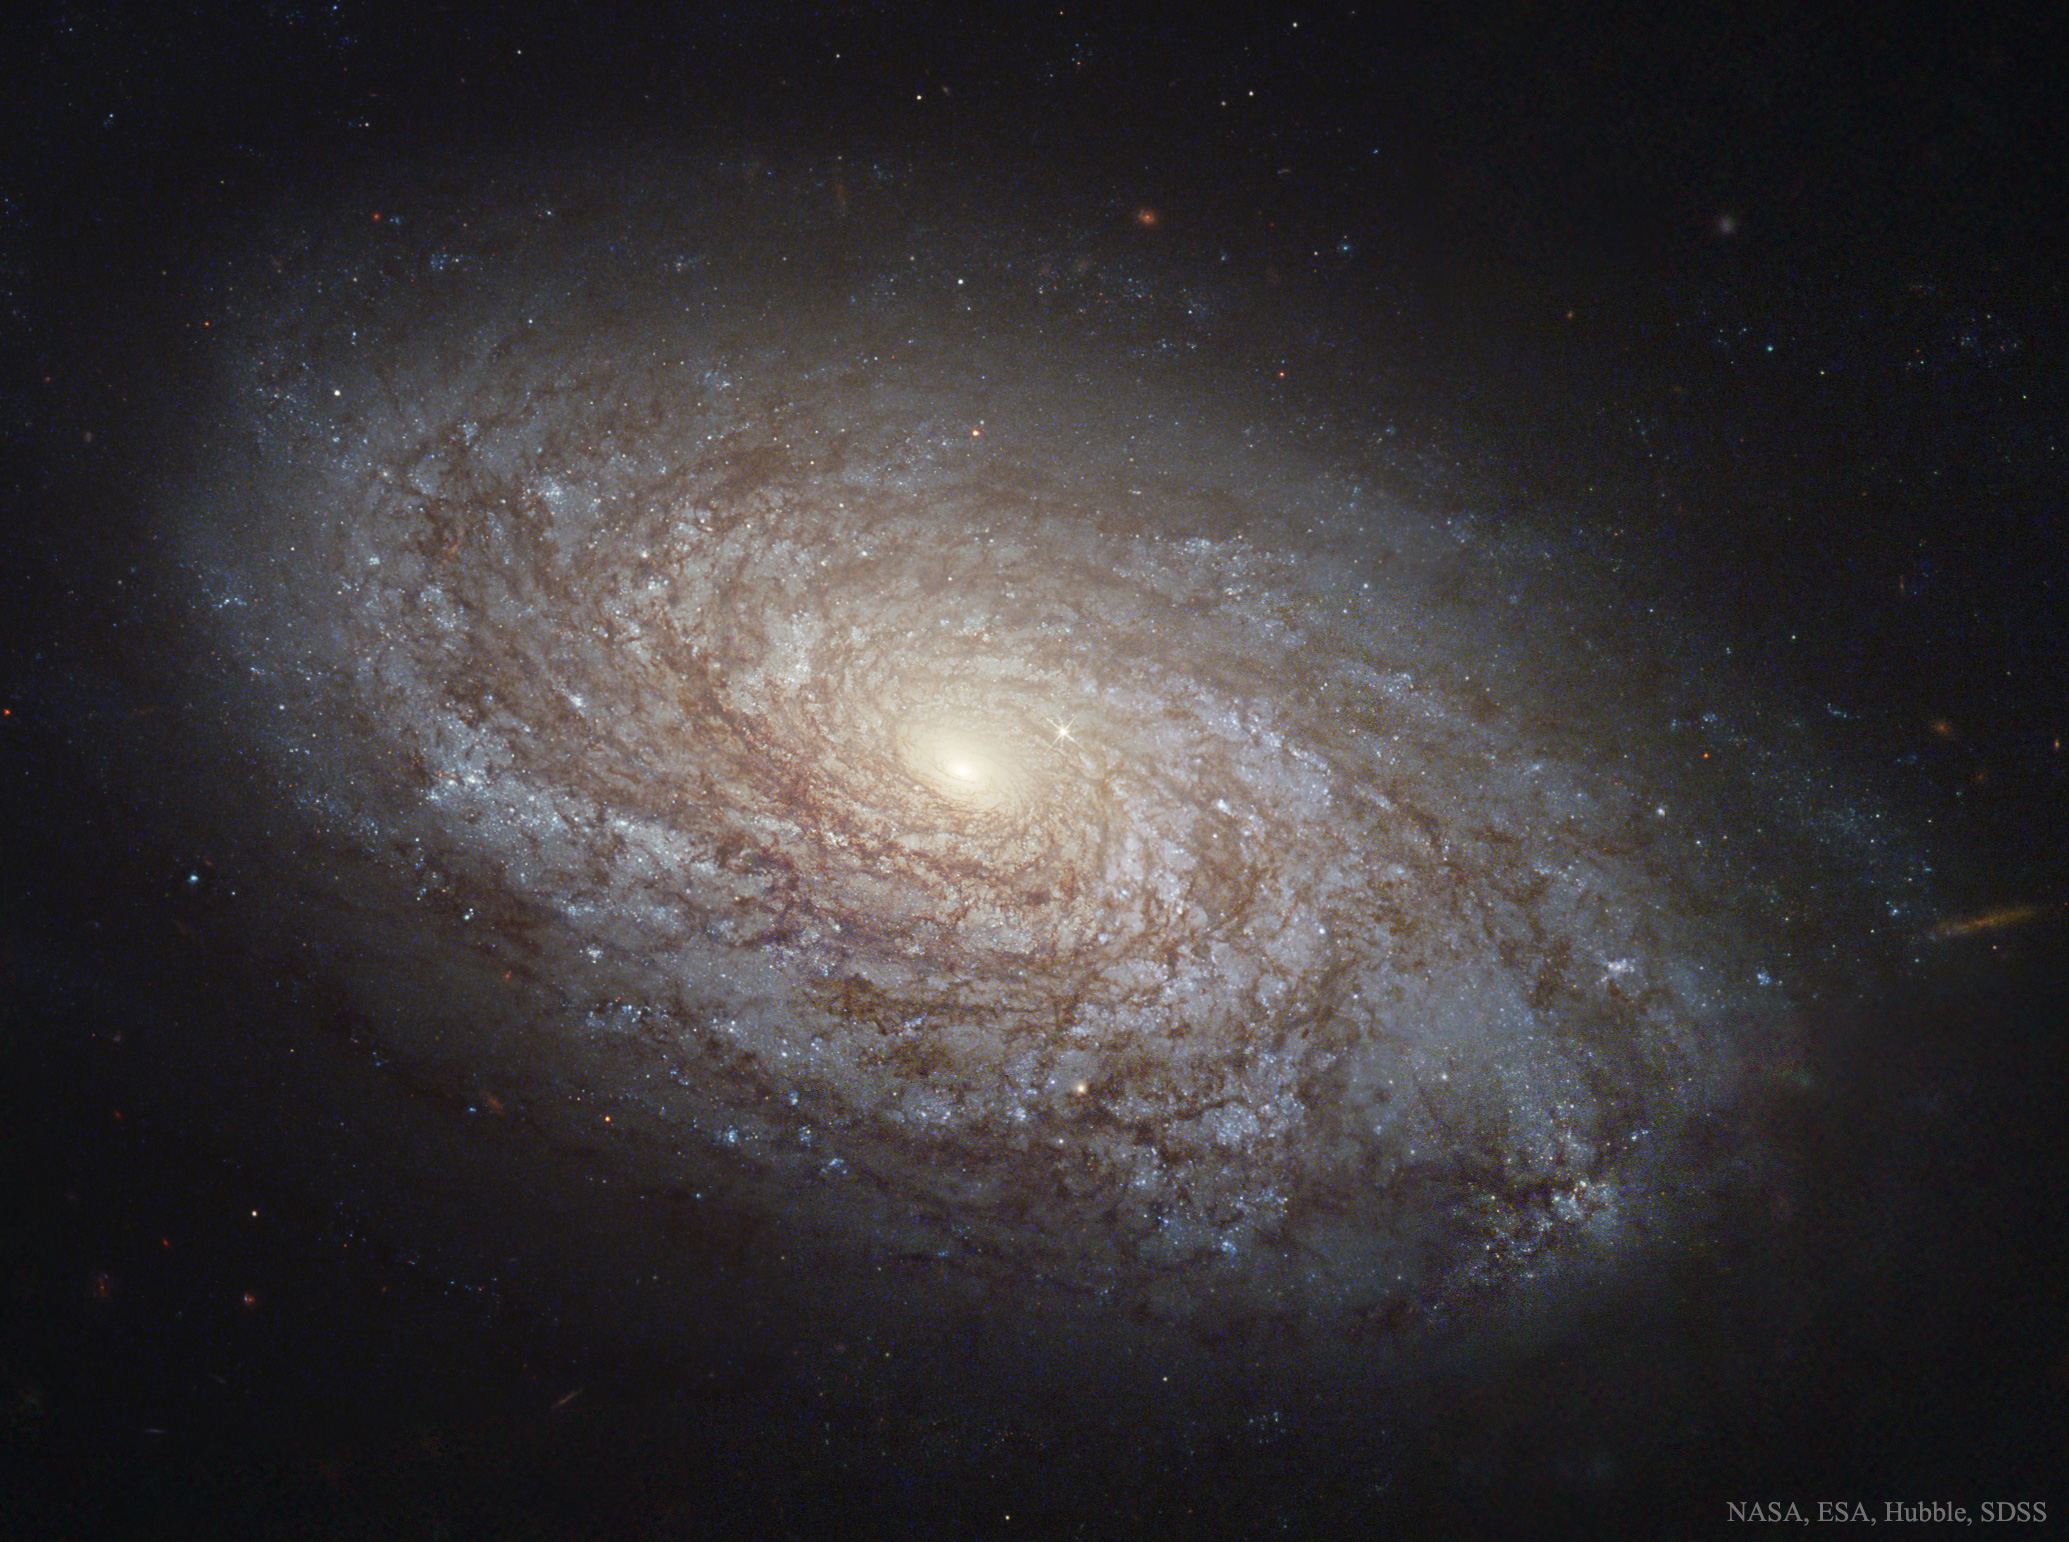
\includegraphics[scale=0.08]{floculenta.jpg}
\caption{Representación artística de una galaxia floculenta.}
\end{center}
\end{figure}
\end{frame}
\begin{frame}{Formación estelar autopropagada}

La teoría de la formación estelar autopropagada podría explicar el origen de estos brazos enmarañados.

\begin{block}{SPSF}
La formación estelar produce supernovas y vientos solares que suscitan más formación estelar. Estas regiones más densas se ven 'apretadas' por la acción de la rotación diferencial. Y esto da lugar a una galaxia de brazos cortos y enmarañados sin simetría apreciable. \cite{cosmo}
\end{block}
\end{frame}
\begin{frame}{Corrimiento al rojo}
Es extraño observar galaxias espirales con un corrimiento al rojo $z > 2$. \cite{corrimiento}

\begin{alertblock}{Causas}

Esto se puede deber a las altas temperaturas del Universo primigenio. También se baraja que nuestros instrumentos no sean lo suficientemente buenos para observar la estructura de estas galaxias.

\end{alertblock}

\begin{figure}[h!]
\begin{center}
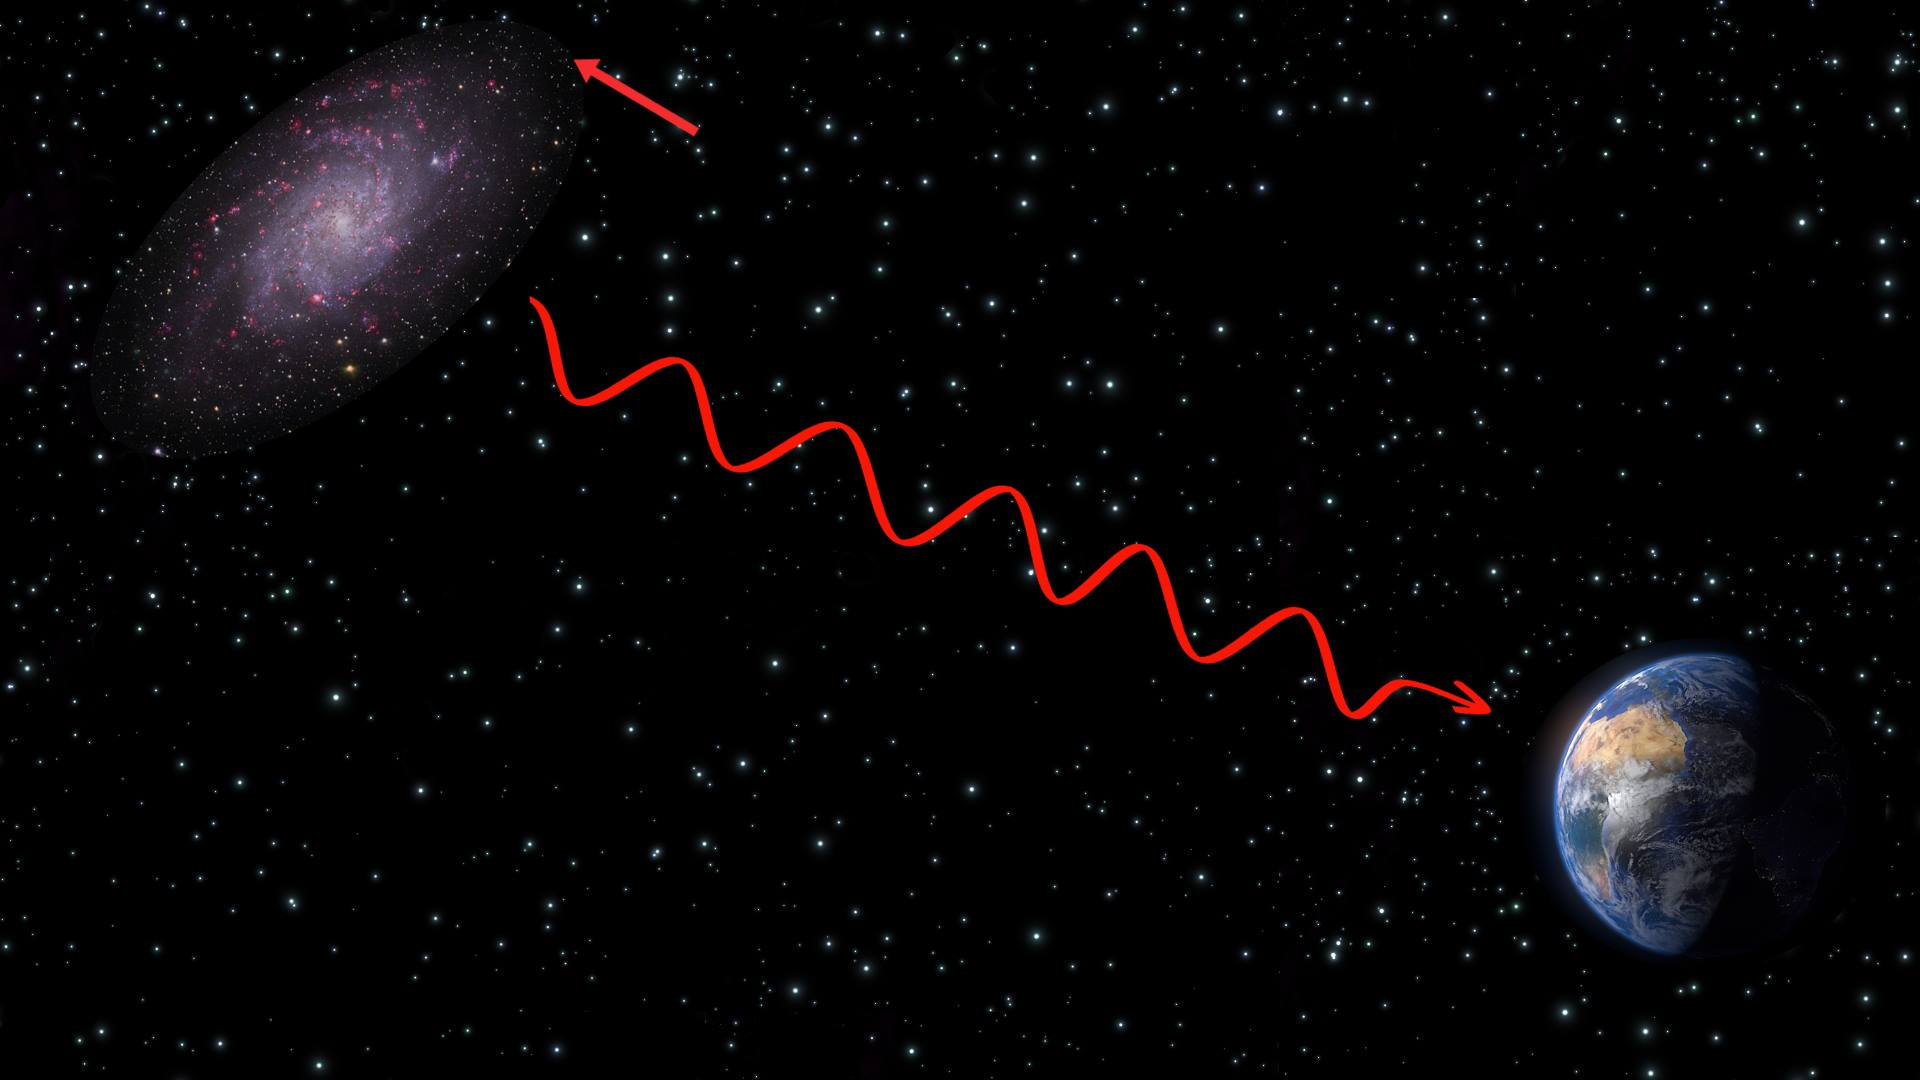
\includegraphics[scale=0.1]{rojo.jpg}
\end{center}
\end{figure}
\end{frame}

\begin{frame}{Un caso excepcional BX442}
\section{Un hecho peculiar}
\begin{exampleblock}{}
La galaxia BX442 tiene un corrimiento al rojo de $z = 2.17$.
\end{exampleblock}
\begin{figure}[h!]
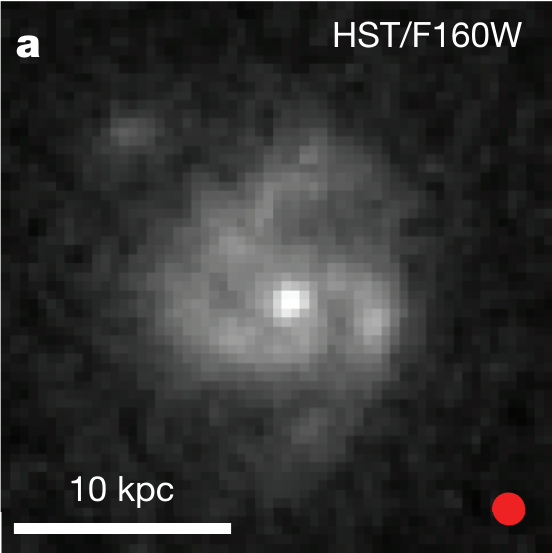
\includegraphics[scale=0.35]{galax1}\hspace{1cm}
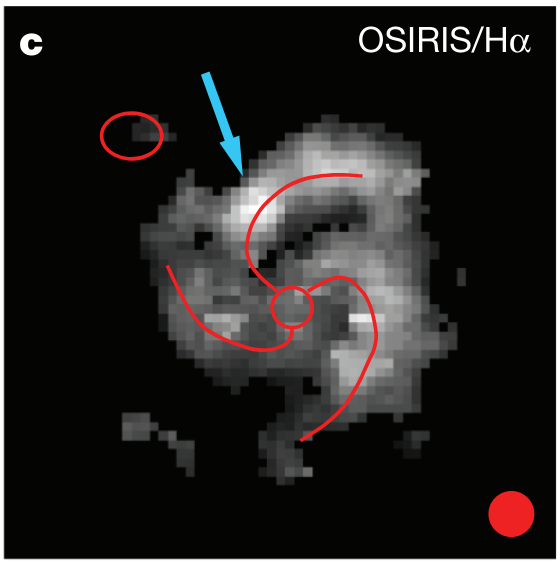
\includegraphics[scale=0.35]{galax2}
\caption{Imagen del Hubble (izquierda) y del OSIRIS (derecha).}
\end{figure}
\blfootnote{Imágenes tomadas por David R. Law}
\end{frame}

\begin{frame}{Conclusión}
\section{Conclusiones}
\begin{block}{Conclusiones}
\begin{itemize}

    \item Hemos utilizado distintos modelos para abordar la formación de galaxias espirales.
    \item Ninguna de las propuestas es definitiva.
    \item Esperamos cambios en el futuro que arrojen luz sobre la formación de estas estructuras.
\end{itemize}
\end{block}
\end{frame}

\begin{frame}{Bibliografía}
\section{Referencias}

\printbibliography

\end{frame}
\end{document}